% fig7_53.tex — 7-64: 耦合振子（三根弹簧 + 两个质量）
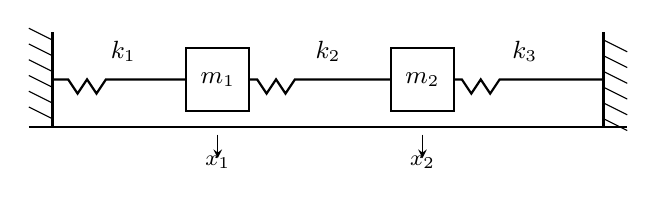
\begin{tikzpicture}[font=\small,>=stealth]
  % 左墙
  \draw[thick] (-2.5,0.6) -- (-2.5,-0.6);
  \foreach \y in {-0.5,-0.3,...,0.5}
    \draw (-2.5,\y) -- (-2.8,{\y+0.15});
  % 右墙
  \draw[thick] (4.5,0.6) -- (4.5,-0.6);
  \foreach \y in {-0.5,-0.3,...,0.5}
    \draw (4.5,\y) -- (4.8,{\y-0.15});
  % 地面
  \draw[thick] (-2.8,-0.6) -- (4.8,-0.6);
  % 左弹簧 k1
  \draw[thick] (-2.5,0) -- ++(0.2,0)
    foreach \i in {1,...,4}{
      -- ++(0.12,{(-1)^\i*0.18})
    } -- (-0.8,0);
  % 物块1
  \draw[thick,fill=white] (-0.8,-0.4) rectangle (0,0.4);
  \node at (-0.4,0) {$m_1$};
  % 中间弹簧 k2（连接两物块）
  \draw[thick] (0,0) -- ++(0.1,0)
    foreach \i in {1,...,4}{
      -- ++(0.12,{(-1)^\i*0.18})
    } -- (1.8,0);
  % 物块2
  \draw[thick,fill=white] (1.8,-0.4) rectangle (2.6,0.4);
  \node at (2.2,0) {$m_2$};
  % 右弹簧 k3
  \draw[thick] (2.6,0) -- ++(0.1,0)
    foreach \i in {1,...,4}{
      -- ++(0.12,{(-1)^\i*0.18})
    } -- (4.5,0);
  % 标注
  \node[above] at (-1.6,0.1) {$k_1$};
  \node[above] at (1,0.1) {$k_2$};
  \node[above] at (3.5,0.1) {$k_3$};
  % 位移标注
  \draw[->] (-0.4,-0.7) -- (-0.4,-1) node[midway,below,font=\footnotesize] {$x_1$};
  \draw[->] (2.2,-0.7) -- (2.2,-1) node[midway,below,font=\footnotesize] {$x_2$};
\end{tikzpicture}
